\documentclass{article}
\usepackage{graphicx}
\usepackage{algorithm}
\usepackage[noend]{algorithmic}
\usepackage{subfigure}
\usepackage{amssymb, amsmath, graphicx, charter, latexsym}
\usepackage{layouts}
\usepackage[letterpaper]{geometry}
\usepackage{enumerate}
\usepackage{epstopdf}
\usepackage{ragged2e}
%\usepackage{times}
\usepackage{mathtools}
%\usepackage[scaled]{helvet}
\usepackage{mathptmx}
\usepackage{verbatim}
\usepackage{listings}
\usepackage{siunitx}
\usepackage{booktabs}
\usepackage{pdfpages}
\usepackage{float}



\lstset{
basicstyle=\ttfamily,
}

\begin{document}

\title{\bf ECEN 689-- Real-Time Wireless Networks: Project 2\\ (Due on 4/1)}
\date{}
\author{%
Ping-Chun Hsieh\\
\texttt{lleyfede@tamu.edu}
\and
Tao Zhao\\
\texttt{alick@tamu.edu}
\and
Dongni Han\\
\texttt{handongni2015@tamu.edu}
}
\maketitle

\section*{Terminology}

In our report, we use ``server'' to denote the WiFi access point (AP), and
``client'' to denote the terminal device such as a mobile phone, a tablet, and
so on. Throughout our simulation, we let node $0$ be the server, and node $1$ be
the client, which correspond to the device A and B in the problem descriptions
respectively.

S-WiFi is the name of our application as well as our project. It stands for
Smart WiFi, or whatever you think it is.

\section*{Simulation Setup}
\begin{table}[htbp]
\centering
    \caption{Parameters of the wireless channel.}
    \vspace{2mm}
    \begin{tabular}{ | l | l | }
    \hline
    Item & Value \\ \hline
    Path loss exponent & 2.0  \\ \hline
    Shadowing deviation & \SI{4.0}{dB} \\ \hline
    Reference distance & \SI{1.0}{m} \\
    \hline
\end{tabular}
\label{table: channel}
\end{table}
Throughout the report, we consider a single wireless link between two devices, say A and B. The transmitter power level is \SI{10}{mW}. We use the shadowing module as the wireless channel. The parameters of the channel are summarized in Table \ref{table: channel}.

\begin{table}[htbp]
\centering
\caption{Parameters of the 802.11b MAC.}
    \vspace{2mm}
    \begin{tabular}{ | l | l | }
    \hline
    Item & Value \\ \hline
    Data rate & \SI{11}{Mb/s}  \\ \hline
    Basic rate & \SI{1}{Mb/s}  \\ \hline
    PLCP data rate & \SI{1}{Mb/s}  \\ \hline 
    Preamble length & \SI{144}{bits} \\ \hline
    Slot time & \SI{20}{\mu s} \\ \hline
    SIFS & \SI{10}{\mu s} \\
    \hline
\end{tabular}
\label{table: mac}
\end{table}

For the medium access control (MAC) layer, we use the 802.11 module built in ns-2. Following the IEEE 802.11b standard, the MAC layer parameters are chosen as in Table \ref{table: mac}.


\section*{Uplink Transmissions with PCF}
\label{section: uplink}



\section{Baseline Policy}
\label{section: baseline}


\frenchspacing In PCF mode, the AP decides which client can transmit: The AP will first send a POLL packet to the selected client. A client can only transmit its packet after it receives the POLL packet from the AP. This allows the AP to have full control over which client transmits. However, there is one problem: Packets arrive at the clients, and the AP cannot know which client has packets for transmission. Baseline policy: At the beginning of each interval, the AP asks each client, one by one, the number of packets that it generates. After this process, the AP also knows the number of packets at each client, and it can make the best decision.


First of all, the server can poll packets or poll data implemented by function \lstinline |command| in the swifi.cc file. Then, the client enables to send number of packets or data to the server implemented by function \lstinline |recv| in the swifi.cc file. Also, we need function \lstinline |scheduleRoundRobin| to let AP ask each client one by one the number of packets that it generates at the beginning of each interval. Then, we need function \lstinline |scheduleMaxWeight| to implement maxweight policy. 

Besides, we define four packet types. 
\begin{table}[h!]
   \centering
   \caption{Data Type}
   \label{tab:table3}
   \begin{tabular}{| l | l |}
      \hline
      Data Type  &  Meaning\\ \hline
      \lstinline |SWiFi_POLL_NUM| & Poll number of packets in uplink\\ \hline 
      \lstinline |SWiFi_PKT_POLL_DATA|  & Poll data packet transmission in uplink\\ \hline 
      \lstinline |SWiFi_PKT_NUM_UL| & Packet in uplink that carries number of packets at client\\ \hline 
      \lstinline |SWiFi_PKT_DATA_UL| & Data packet in uplink(client to server)\\  
     \hline
   \end{tabular}
\end{table}
 
  
What's more, four poll states are defined below. 
\begin{table}[h!]
   \centering
   \caption{Poll State}
   \label{tab:table4}
   \begin{tabular}{| l | l |}
      \hline
      Poll State  &  Meaning\\ \hline
      \lstinline |SWiFi_POLL_NONE| & Poll nothing\\ \hline 
      \lstinline |SWiFi_POLL_NUM|  & Poll num of packets\\ \hline 
      \lstinline |SWiFi_POLL_DATA| & Poll data\\ \hline 
      \lstinline |SWiFi_POLL_IDLE| & Idle\\  
     \hline
   \end{tabular}
\end{table}
     
\begin{figure}[H]
\centering
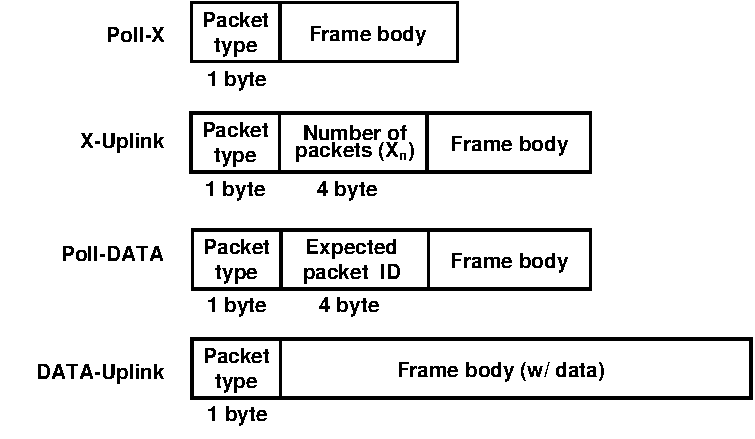
\includegraphics[scale=0.6]{header.pdf}
\caption{Packet Type}
\end{figure}

However, there are still some issues. Look at Figure 2, there is a possibility that AP Poll-X or a client poll X1 is not delivered successfully. Our method is retransmit Poll-X until the AP receives Xn. And we just set Xn = 0 if poll X does not deliver successfully. 

\begin{figure}[H]
\centering
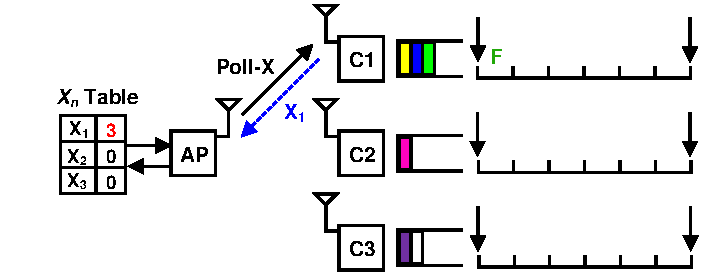
\includegraphics[scale=0.8]{discussion_1.pdf}
\caption{Issue 1}
\end{figure}

Look at Figure 3, how does a client know the DATA packet is delivered? Do we need an application-layer ACK for AP?  We put expected packet ID in Poll-DATA packets so that the client knows its last packet is delivered when AP asks its next packet. Thus, we needn't an application-layer "ACK" for AP. 

\begin{figure}[H]
\centering
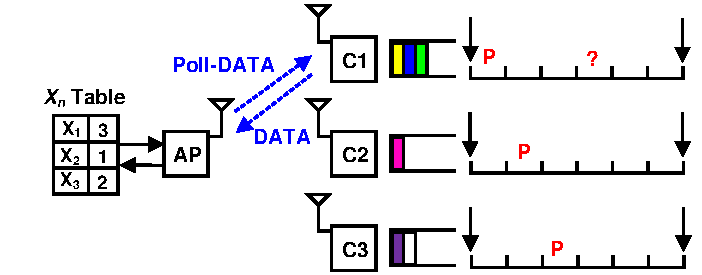
\includegraphics[scale=0.8]{discussion_2.pdf}
\caption{Issue 2}
\end{figure}

Look at Figure 4, what does "Xn" mean for non-real-time traffic? The answer is that the queue length equals total number of packets generated by a client minus total delivery of data packets from a client. So the max-weight policy chooses a client with the largest channel reliability times current queue length. 

\begin{figure}[H]
\centering
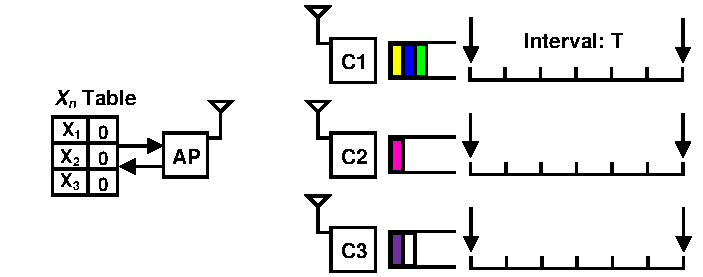
\includegraphics[scale=0.8]{discussion_3.pdf}
\caption{Issue 3}
\end{figure}


\section{Implementation in NS-2}
\label{section: ns2}
In our SWiFi project, the way we implement baseline policy is described as follows. 

In the \lstinline |command| function in swifi.cc

When the system captures a string called  \lstinline |server| indicating that it is a server(AP). If the value of  \lstinline |do_pull_num|  is true,  \lstinline |poll_state_|  will be set to  \lstinline |SWiFi_POLL_NUM|. Otherwise, when the value of  \lstinline |do_pull_num|  is false,   \lstinline |poll_state_|  will be set  \lstinline |SWiFi_POLL_DATA|. 


When the system captures a string called  \lstinline |poll|, tcl will print an error: only server AP can poll if it's not a server. If it's a server, the server(AP) will ask each client one by one using function \lstinline |scheduleRoundRobin| when the \lstinline |poll_state_| is  \lstinline |SWiFi_POLL_NUM|. And we set the packet type to \lstinline |SWiFi_PKT_POLL_NUM|, store current time and send the new packet. Otherwise, the server(AP) will use maxweight policy to schedule clients using function \lstinline |scheduleMaxWeight| when the \lstinline |poll_state_| is  \lstinline |SWiFi_POLL_DATA|. And we set the packet type to \lstinline |SWiFi_PKT_POLL_DATA|, store current time and send the new packet. Besides, there is one special condition that no more client is left in one interval (\lstinline |target_| is true). In this case, \lstinline |poll_state_| will be set to \lstinline |SWiFi_POLL_IDLE|.


When the system captures a string \lstinline |boi| meaning at the beginning of each interval, the system will set \lstinline |target_| to NULL. If  \lstinline |realtime_|  is true indicating it is real-time traffic, we need clear number of data packets of all clients at the beginning of each interval. 

In the  \lstinline |recv| function in swifi.cc

When a client receives a packet type \lstinline |SWiFi_PKT_POLL_DATA| transmitted by a server, we save the old packet's send time, discard the old packet, create a new packet, set new send time and send this new packet to the server(AP). 
When a client receives a packet type \lstinline |SWiFi_PKT_POLL_NUM| transmitted by a server, we set the data type to \lstinline |SWiFi_PKT_NUM_UL| meaning that it is uplink packet with numbers of packets at client, set new send time and send this new packet to the server(AP).
When a server receivers  a packet type \lstinline |SWiFi_PKT_NUM_UL| transmitted by a client, the current queue length is equal to the number of data packets generated minus the number of data packets received. For real-time traffic, the current queue length is equal to the number of data packets generated.  

For Real-time traffic: At the beginning of each interval, we need clean queues of all clients cause we don't need store the queue length last interval. The current queue length just equals random number of packets at the beginning of each interval. If all packets miss its deadline, we just drop those packets.

For Non-real-time traffic:  If all packets miss its deadline, we don't drop those packets. We need store the queue length last interval. The current queue length is equal to total number of data packets generated by clients minus total number of delivery data packets from clients. 

We consider this system as a state machine. But NS-2 doesn't provide a state machine. We just define some enum to define these states. 

\begin{figure}[H]
\centering
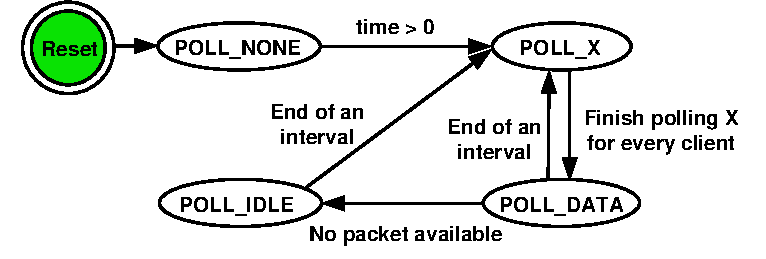
\includegraphics[scale=0.8]{state_machine.pdf}
\caption{State Machine}
\end{figure}


\section{Simulation Results}
\label{section: simulation}
\subsection{Symmetric System with 2 Clients}
We assume T=10 intervals =100ms, channel reliability p1 = p2 = 1

For non-real-time traffic, according to Figure 6, \lstinline |Nmax| ranges from 1 to 12. We can conclude that polling reduces channel capacity. 

\begin{figure}[H]
\centering
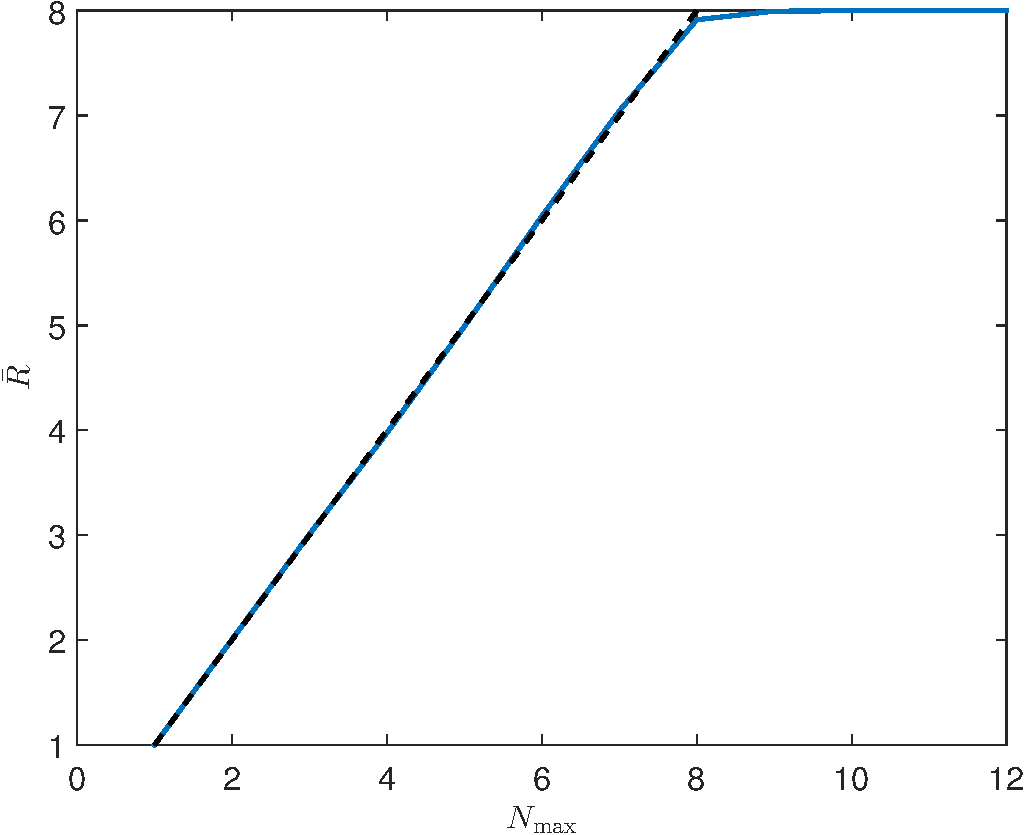
\includegraphics[scale=0.5]{nonrealtime_throughput_randmax.pdf}
\caption{Non-real-time traffic and symmetric system with 2 clients}
\end{figure}

For real-time traffic, according to Figure 7, \lstinline |Nmax| ranges from 1 to 20. We can conclude that packet deadline reduces the capacity further cause packets are dropped if they miss their deadline. 

\begin{figure}[H]
\centering
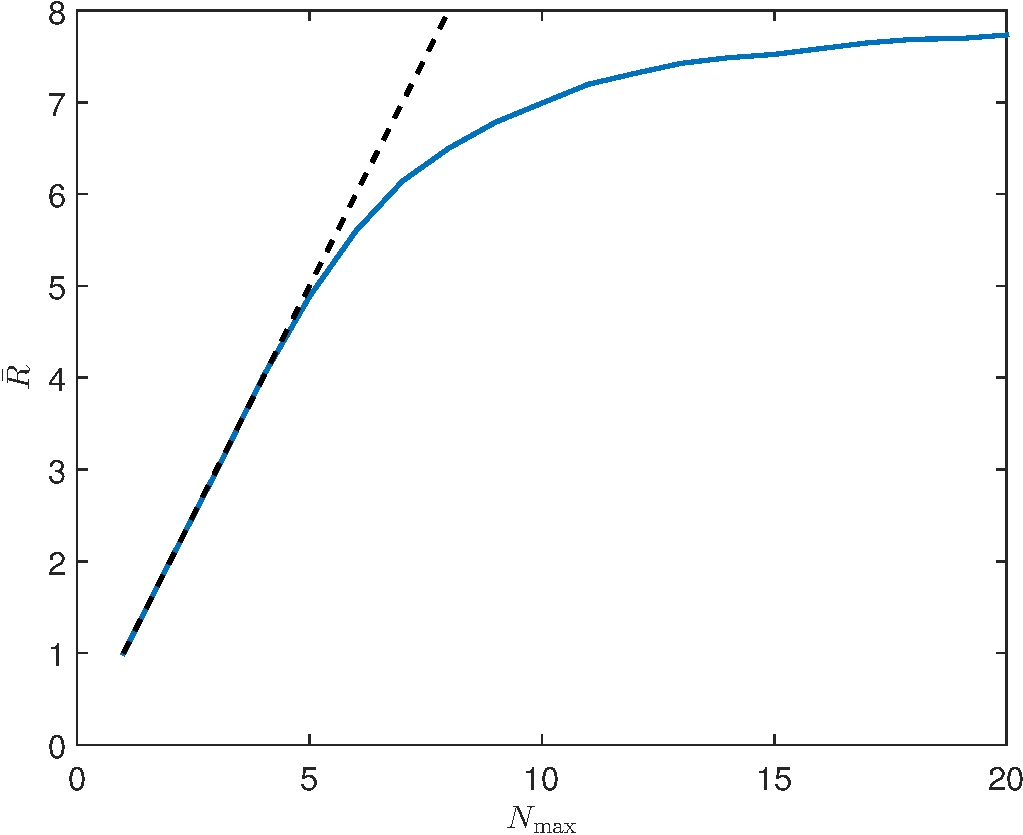
\includegraphics[scale=0.5]{realtime_throughput_randmax.pdf}
\caption{Real-time traffic and symmetric system with 2 clients}
\end{figure}

\subsection{Asymmetric System with 2 Clients}
We assume N = 2, channel reliability p1 = p2 = 0.57 (distance 1000m).

For non-real-time traffic, according to Figure 8, T ranges from 4 to 16. We can conclude that interval should be long enough to guarantee deliveries. If interval is too short, AP will not have enough time slots to poll data to clients. 

\begin{figure}[H]
\centering
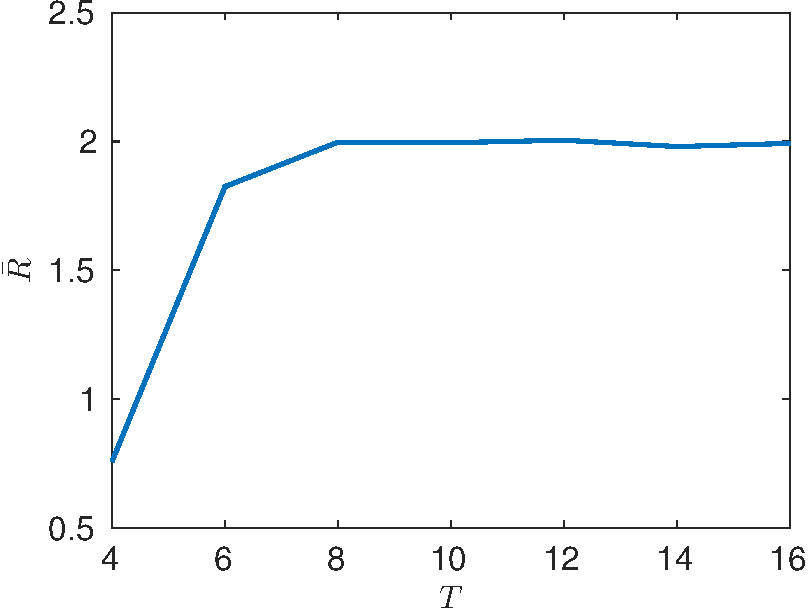
\includegraphics[scale=0.7]{nonrealtime_throughput_T.pdf}
\caption{Non-real-time traffic and Asymmetric system with 2 clients}
\end{figure}

For real-time traffic, according to Figure 9, T ranges from 4 to 16. We can conclude that interval should be longer so that packets cannot expire and they won't miss their deadline. 

\begin{figure}[H]
\centering
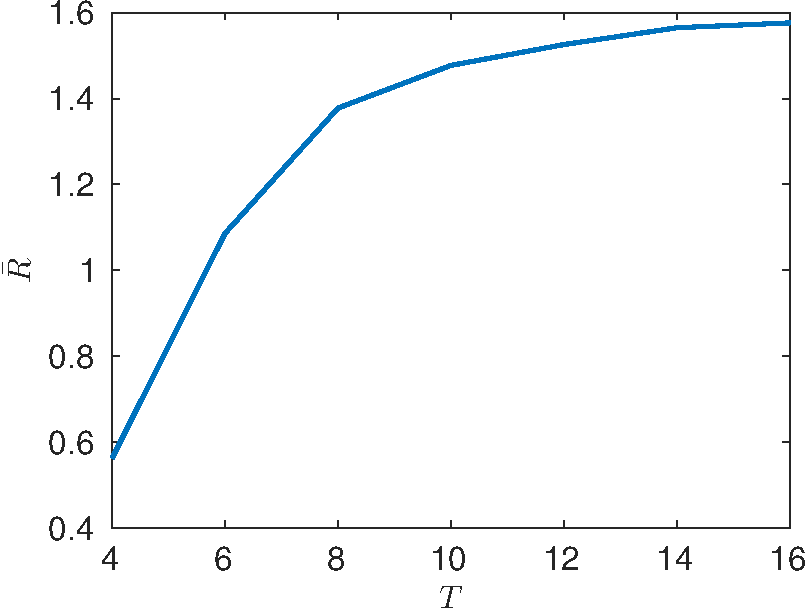
\includegraphics[scale=0.7]{realtime_throughput_T.pdf}
\caption{Non-real-time traffic and Asymmetric system with 2 clients}
\end{figure}

\subsection{System with N Clients}
We fix T = 10, channel reliability p1 = p2 = 0.57 (distance 1000m).

For non-real-time traffic, according to Figure 10, N ranges from 1 to 5. We can conclude that channel performance degrades severely with more clients. So the baseline policy is not suitable for a large number of clients cause it spends many time slots polling. 

\begin{figure}[H]
\centering
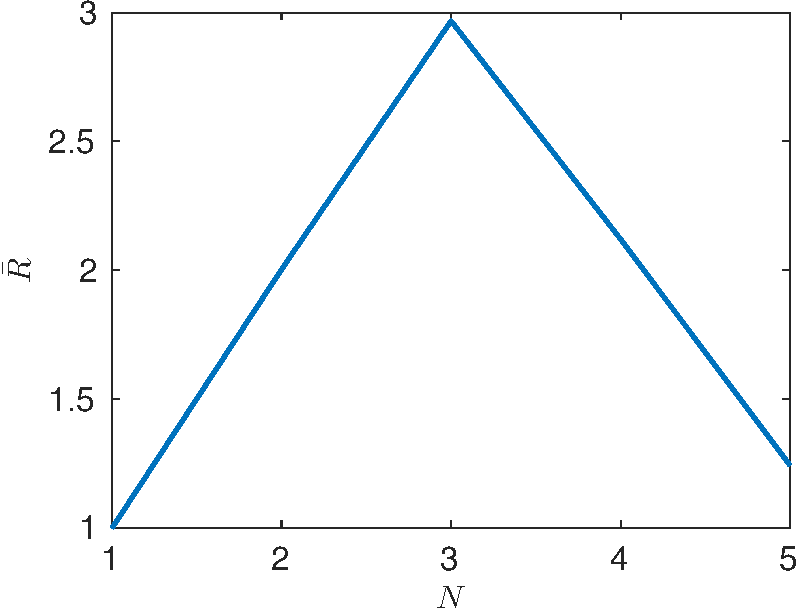
\includegraphics[scale=0.7]{nonrealtime_throughput_N.pdf}
\caption{Non-real-time traffic with fixed T = 10}
\end{figure}

For real-time traffic, according to Figure 11, N ranges from 1 to 5. We can conclude that channel performance is even worse compared with non-real-time traffic and it also degrades with more clients. The reason is that packets will expire if they miss its deadline.  

\begin{figure}[H]
\centering
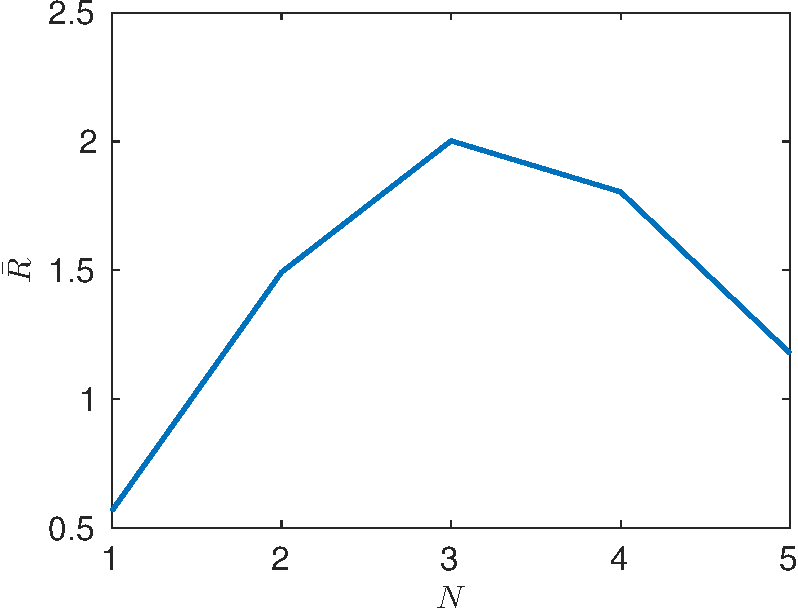
\includegraphics[scale=0.7]{realtime_throughput_N.pdf}
\caption{Real-time traffic with fixed T = 10}
\end{figure}

\section{Conclusion}
The system has a simple polling scheme and the server is work-conversing in scheduling clients based on maxweight policy. However, the channel utilization for data packets is low and it is not practical when the number of clients is large or the interval is small. The reason is that the system will spend many time slots on polling when it has a large number of clients N. Also, the system will not have enough time to poll if it has small interval T. 

All in all, the baseline policy incus huge overhead. So we need a smarter policy.

\end{document}